In der Praxis sollten ein Cisco-Router (Modell unbekannt, zwei GigabitEthernet-Ports) und ebenfalls ein Cisco-Switch entsprechend verkabelt und konfiguriert werden. Ebenfalls war eine IP-Konfiguration von zwei verschiedenen Endgeräten durchzuführen. Zusätzlich wurde noch ein Access-Point eingerichtet, sodass auf das Netzwerk auch kabellos zugegriffen werden kann. Die Verkabelung der einzelnen Komponenten wurde entsprechend \ref{fig:netzplan_physisch} durchgeführt.

\begin{figure}[h]
	\centering
	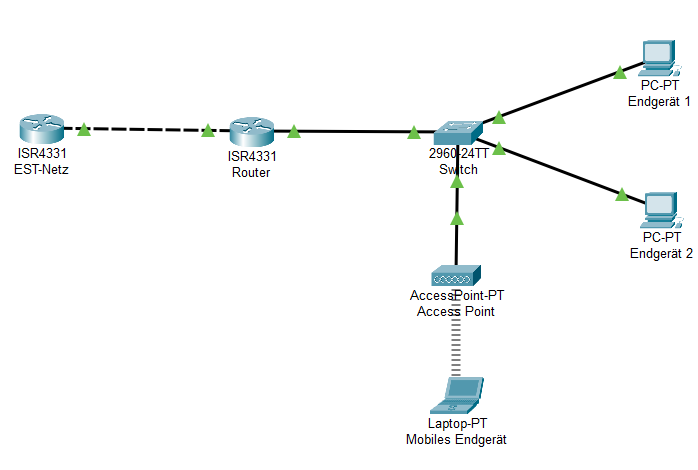
\includegraphics[width=15cm]{images/Netzplan_physisch.png}
	\caption[Praktischer Netzplan]{Netzplan für die praktische Umsetzung}
	\label{fig:netzplan_physisch}
\end{figure}